\documentclass{article}

\usepackage[utf8]{inputenc}
%\usepackage{fancyhdr}
\usepackage[letterpaper, portrait, margin=1.7in]{geometry}
\usepackage{natbib}
\usepackage{graphicx}
\usepackage{listings}
\usepackage{blindtext}
\usepackage{enumitem}
\usepackage{pgf-umlsd}
\usepackage{tikz}
\usepackage{float}

\title{
    Instant Messenger Protocol\\
    \large IP Network Fundamentals\\
    IMT Atlantique
}

\author{
    Jesús Alberto Polo\\ \texttt{jesus.pologarcia@imt-atlantique.net}\\\\
    Erika Tarazona\\ \texttt{erika.tarazona@imt-atlantique.net}
}

\date{February, 2017}

\begin{document}

\maketitle

\section{Abstract}
Instant Messenger Protocol offers to upper layer a way to exchange written messages in a reliable way, using User Datagram Protocol (UDP) at transport layer. This protocol specification defines a minimum set of requirements to be able to implement the different elements that interacts within the protocol, namely the client and the server. The protocol scope as well as the operation design are defined based on an ensemble of requirements previously given.   

\tableofcontents
\cleardoublepage

\section{Introduction}

This document describes the Instant Messenger Session Protocol Specification, the protocol operates at session layer in OSI reference model, it serves to a client-server oriented application in session management tasks and operations.\\

A session is considered an exchange of data between an association of participants. Instant Messenger Protocol permits exchanging of messages among clients connected to a Server. Those clients belong to a group public or private managed by the aforementioned server.\\

This document is organized to give firstly an operation overview of the protocol, followed by a description of the component and their roles in protocol operation. A section with messages details deeps down into the specific protocol operation, and a section with scenario flows illustrates the message exchange between the different components.

\section{Protocol Operation Overview}

Instant Messenger allows users to exchange short written messages interactively through a centralized service allocated in a server or directly between users. The upper layer uses a session protocol for transactional control operations at that layer, described as Instant Messenger Session Protocol.

\subsection{Main Components}

\subsubsection{Server}

It is the central element in the architecture, it manages all the control tasks performed in order to establish the sessions, invitations to groups, user updates as well as disconnections are treated by it. The communication between users can be centralized or decentralized. In centralized, the server proxies out client-client(s) messages. Oppositely in decentralized mode, the server stays out of messages exchange between users but it still manages the control messages.

\subsubsection{Client}

A client is an element in the architecture representing the user, it generates messages and share them with other members in its group, along with other control messages exchanged with the server. A client has a unique ID given by the server at the begin of the connection. The maximum number of users connected in the system is 4094.

\subsubsection{Groups}

Groups are pools where the clients belong to and can exchange messages in a multicast way, there are two types of groups: public group, just one exist, and private groups, many of them can exist. At the first place clients are put by default into the public group, then if they receive an invitation to join or they want to create another private group, a procedure is handled by the server to accomplish this task, it will be explained later in the specification. The maximum number of groups in the system, including the Public Group, is 4092. This protocol will never reach this number of groups since a group is formed when there are at least two clients. However it is necessary if more than half of the users want to create a new private group at the same time, because the server has to assign temporal Group ID for each new group.

\begin{figure}[t]
\centering
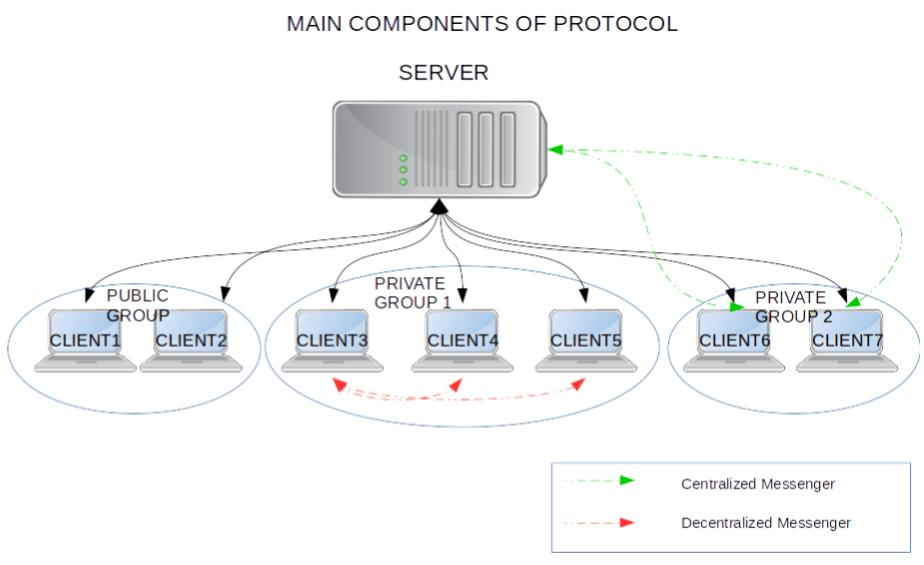
\includegraphics[width=9cm, height=6cm]{Maincomponents.jpg}
\caption{Main Components of Instant Messenger Protocol}
\label{fig:Maincomponents}
\end{figure}

\subsection{Model of Operation}

To outline the general operation, first a client initiates a connection with the server who puts it into a default group called Public Group, and assigns a Client ID to identify it. Once the connection is established, the client ask for the list of clients, and the server send the list of current connected clients indicating their Client IDs, Group ID (if equal to 1 is public, otherwise is private), socket address (IP address and port), and username.\\

It is important to underline that the socket address (IP address and port) is needed because in decentralized mode the users need to communicate directly, and the server (who is the one that has this information) is out of communication, therefore clients need to know the socket of each others to communicate directly.\\

When a client sends a message to the group, it is handled by the server who forwards it to other members of the group when the operation is centralized mode, all members will receive the message which contains header (with Client ID of the sender) and data. On the other hand, in decentralized mode, a client sends directly a message to all other members of the group.\\

At lower layer, the transportation is managed by User Datagram Protocol (UDP) \cite{3}, as consequence message acknowledgement is performed by the session layer so that it can guarantee connection reliability. For this purpose Stop-and-Wait ARQ mechanism is used, where an acknowledgement for each type of message confirms its reception when there is no explicit response.\\

Once a message is sent, a timer is activated and the party waits for the Acknowledgement message or a message that serves as an acknowledgement. When it receives the acknowledgement, the timer is reseated, by default the timer is set to 500ms, based on some guidelines in \cite{1}, \cite{2}. If the timer expires the message must be retransmitted and the process is repeated sveral times (this protocol recommends up to 5 times), after that if no acknowledgement is received the message is discarded and the user is considered as out of the system (forced disconnection).\\

When a client needs to disconnect just asks the server for it. The server is responsible for confirming and updating the clients data base changes to other members. In the same way, when a forced disconnection is detected, the server will remove the user from the system and it will send an update to the other users.\\

A client can be invited to other group, this task is handled by the server when an invitation request is issued from one client to another client. Once the client accepts the invitation it will not further receive messages from the former group but just the ones interchanged into the new group. Additionally, the client can not send messages to former group's members anymore, unless it is an invitation to join another group, keeping in mind that server is in the middle the whole time. This message is also issued when a client requests a group creation including the client IDs of the invited users, thus the server sends an Group Invitation Request to those users.\\

%explicar como se maneja el tema del timer y la retransmision

\begin{verbatim}
               +-------------+
               | Application |              Application Layer
               +------+------+
                      |
        +-------------+--------------+
        | Instant Messenger Protocol |      Session Layer
        +-------------+--------------+
                      |
          +-----------+------------+
          | User Datagram Protocol |        Transport Layer
          +-----------+------------+
                      |
            +---------+---------+
            | Internet Protocol |           Network Layer
            +---------+---------+
                      |
          +-----------+------------+
          | Local Network Protocol |        Link Layer
          +------------------------+
          
                        Protocol Relationships
\end{verbatim}

\subsection{Operation Modes}

The protocol offers two communication options for clients, namely the centralized mode and decentralized mode, where client-server interaction changes depending on which mode is on.

\subsubsection{Centralized}

In centralized mode, the server takes care of all packets shared in the network, even those that are data, it is always amid the connection. In this mode the server receives messages coming from clients and resend them to all group members, using the existing connection. Server is also responsible for acknowledge management, and for resending information when an error in transmission occurs.

\subsubsection{Decentralized}

In this mode the server is there for control and communication establishment, nonetheless once the connection between two or more clients inside a group is done, the server leaves the communication and clients exchange messages directly among them.\\

When a client (Client A) asks for a group creation with this mode on, the server assigns the Group ID and sends it to that client in option data field when, at least, one user accepted a Group Invitation Request.\\

Once the connection is fully established between them, clients can exchange messages and acknowledgements without passing throughout the server. When a client inside the group wants to invite a client outside the group, this control task will be performs by the server, who will forward the invitation to the outsider and will be managing the whole processes until the invited client becomes a member of the group. In the same way, when a client wants to leave the group or the system, the server will be the responsible for handling these tasks.\\

When a client tries to send a message to another client in its group and it detects that the client suffered a forced disconnection (it disconnected without sending any Disconnection Request), the sender will remove this client from its list. The server will realize the forced disconnection when sending a message control or update.

\clearpage

\section{Protocol Header}

\begin{verbatim}
 0                   1                   2                   3  
 0 1 2 3 4 5 6 7 8 9 0 1 2 3 4 5 6 7 8 9 0 1 2 3 4 5 6 7 8 9 0 1
+-+-+-+-+-+-+-+-+-+-+-+-+-+-+-+-+-+-+-+-+-+-+-+-+-+-+-+-+-+-+-+-+
|   Type  |R|S|A|   Source ID   |    Group ID   | Header Length |
+-+-+-+-+-+-+-+-+-+-+-+-+-+-+-+-+-+-+-+-+-+-+-+-+-+-+-+-+-+-+-+-+
|               |                    Options                    |
+-+-+-+-+-+-+-+-+-+-+-+-+-+-+-+-+-+-+-+-+-+-+-+-+-+-+-+-+-+-+-+-+
\end{verbatim}

\begin{description}[align=left]
    \item [Type:] 5 bits 
    \begin{flushleft}
        The Type field identifies the message and it is used to know the structure of the options field and whether any data is sent from upper layers.
        \begin{itemize}
            \item[--] Values from 0x00 to 0x10 has been assigned which makes 17 different types in total.
            \item[--] Values from 0x11 to 0x1F has been reserved for future types.
        \end{itemize}
    \end{flushleft}
    
    \item [Reserved:] 1 bit
    \begin{flushleft}
        The Reserved field is reserved for future use, new flags could be created by using these reserved bits.
    \end{flushleft}
    
    \item [Sequence:] 1 bit
    \begin{flushleft}
        The Sequence field is used to differentiate consecutive messages, where 0 and 1 as possible values, and it changes when a new message is sent. Since this protocol uses Stop-and-Wait ARQ, this field is required for knowing which message is being acknowledged. When Acknowledgement flag is set to 1, that message is acknowledging the value in this field.
    \end{flushleft}
    
     \item [Acknowledgement:] 1 bit
    \begin{flushleft}
        The acknowledgement bit is set to 1 to acknowledge a previous message. It was conceived as a flag to indicate that a particular type of message (indicated in Type field) is acknowledged by this message, considering that protocol use stop and wait to guarantee connection reliability. In this way there is not need of creating an ACK type of messages for each type of message.
    \end{flushleft}
    
    \item [Source ID:] 8 bits
    \begin{flushleft}
        The Source ID field indicates the unique ID of the sender. This number is given by the server to the client during the initial connection negotiation. We have chosen 8 bits to assure at least 250 users and also to suit the header length so that it can form blocks of bytes when combine with group ID field.
        \begin{itemize}
            \item[--] Source ID equals 0 cannot be assigned to or used by any user because it is reserved for situations when client ID doesn't exist yet, it isn't need or the server sends the message.
            \item[--] Source ID varies between 1 and 255 for any user. Note that the server does not need a Source ID.
        \end{itemize}
        
    \end{flushleft}
    
    \item [Group ID:] 8 bits
    \begin{flushleft}
        The Group ID field indicates the unique ID of the destination group because messages are in most of cases addressed to a group. I can be the Public Group or any Private group and also it can be centralized or decentralized. The 12 bits length was chosen for the same reason of source ID. This field is used by all receivers to check if the message was sent to them, otherwise it will be discarded.
        \begin{itemize}
            \item[--] Group ID equals 0 cannot be assigned to neither used by any group because it is reserved for exceptional situations.
            \item[--] Group ID equals 1 is reserved to the Public Group. 
            \item[--] Group ID equals 255 is reserved to the broadcast messages. 
            \item[--] Group ID varies between 2 and 254 for any private group.
        \end{itemize} 
    \end{flushleft}
    
    \item [Header Length:] 16 bits
    \begin{flushleft}
        This field contains the header length including options, in bytes, and it never contains the length of the data from upper layers. Note that the minimum value for a header is 5 bytes. When the value is greater that 5 bytes, optional fields are read as part of the header and the contained information is treated depending on the type of message. This field helps the protocol to know how far to read header, after that point the protocol knows that the contain corresponds to payload.
    \end{flushleft}
    
    \item [Options:] variable
    \begin{flushleft}
        The options field is conceived to carry control information that is not present or needed in all type of messages. Its structure varies depending on the type of the message. Options field details are explained in each message.
    \end{flushleft}
    
\end{description}

\section{Protocol Messages}

\subsection{Connection Request}
Connection request message is sent by the client to initiate a session with the server. The following diagram illustrates the header structure with options corresponding to this type of message.
\clearpage
\begin{verbatim}  
 0                   1                   2                   3  
 0 1 2 3 4 5 6 7 8 9 0 1 2 3 4 5 6 7 8 9 0 1 2 3 4 5 6 7 8 9 0 1
+-+-+-+-+-+-+-+-+-+-+-+-+-+-+-+-+-+-+-+-+-+-+-+-+-+-+-+-+-+-+-+-+
|   Type  |R|S|A|   Source ID   |    Group ID   | Header Length |
+-+-+-+-+-+-+-+-+-+-+-+-+-+-+-+-+-+-+-+-+-+-+-+-+-+-+-+-+-+-+-+-+
|               |                                               |
+-+-+-+-+-+-+-+-+                                               +
|                            Username                           |
+               +-+-+-+-+-+-+-+-+-+-+-+-+-+-+-+-+-+-+-+-+-+-+-+-+
|               |
+-+-+-+-+-+-+-+-+
\end{verbatim}
\begin{description}[align=left]
    \item [Type:] 0x00
        
    \item [Reserved:] 0x0
        
    \item [Sequence:] Sequence number
    
    \item [Acknowledgement:] 0x0
    
    \item [Source ID:] 0x00
    \begin{flushleft}
        In this type of message, the value of source ID is initially 0 because the client does not have assigned any source ID.
    \end{flushleft}
    
    \item [Group ID:] 0x00
    \begin{flushleft}
        The Group ID remains 0 in this message for the reason as source ID, initially the client does not know the group ID it belongs to.
    \end{flushleft}
        
    \item [Header Length:] 0x000D

    \item[Options:] (The size is equal to 8 bytes.)
    \begin{itemize}
        \item[--]\textbf{Username:} This field contents the string given by the user, it can content any ASCII character. The username must be different for each user, it is not possible to connect with a username already taken. The length of this field is 8 bytes, upper layer will manage the filling of non-used bytes (e.g. user chooses an username shorter that 8 characters) to simplify the lecture of this field .
    \end{itemize}
\end{description}

\subsection{Connection Accept}
Connection Accept message is sent by the server to confirm a initial session connection with the client as result of a Connection Request.
\clearpage
\begin{verbatim}  
 0                   1                   2                   3  
 0 1 2 3 4 5 6 7 8 9 0 1 2 3 4 5 6 7 8 9 0 1 2 3 4 5 6 7 8 9 0 1
+-+-+-+-+-+-+-+-+-+-+-+-+-+-+-+-+-+-+-+-+-+-+-+-+-+-+-+-+-+-+-+-+
|   Type  |R|S|A|   Source ID   |    Group ID   | Header Length |
+-+-+-+-+-+-+-+-+-+-+-+-+-+-+-+-+-+-+-+-+-+-+-+-+-+-+-+-+-+-+-+-+
|               |   Client ID   |
+-+-+-+-+-+-+-+-+-+-+-+-+-+-+-+-+
\end{verbatim}
\begin{description}[align=left]
    \item [Type:] 0x01
    
    \item [Reserved:] 0x0
    
    \item [Sequence:] Sequence number
    
    \item [Acknowledgement:] 0x0
    
    \item [Source ID:] 0x00
    \begin{flushleft}
        This field remains 0 since the server pass the source ID information to the client in optional data of this message, after processing the message the client is aware of the new client ID assigned by the server and can use it.
    \end{flushleft}
    
    \item [Group ID:] 0x00
    \begin{flushleft}
        This field also remains 0 since the client does not belong yet to any group, after the connection is fully established this field will contain the group ID by default which is Public Group (with ID 0x01).
    \end{flushleft}
    
    \item [Header Length:] 0x0006
    
    \item[Options:] (The size is equal to 1 byte.)
    \begin{itemize}
        \item[--]\textbf{Client ID (8 bits):}
        This field will carry the client ID assigned by the server. The client reads this value and uses it in future messages as its source ID.
    \end{itemize}
\end{description}

\subsection{Connection Reject}
Connection reject message is sent by the server when there is a problem to establish the initial connection with the client. The server generates an error code when the maximum number of user is reached or when the user has chosen a username that was already taken.

\begin{verbatim}  
 0                   1                   2                   3  
 0 1 2 3 4 5 6 7 8 9 0 1 2 3 4 5 6 7 8 9 0 1 2 3 4 5 6 7 8 9 0 1
+-+-+-+-+-+-+-+-+-+-+-+-+-+-+-+-+-+-+-+-+-+-+-+-+-+-+-+-+-+-+-+-+
|   Type  |R|S|A|   Source ID   |    Group ID   | Header Length |
+-+-+-+-+-+-+-+-+-+-+-+-+-+-+-+-+-+-+-+-+-+-+-+-+-+-+-+-+-+-+-+-+
|               |E|   Padding   |
+-+-+-+-+-+-+-+-+-+-+-+-+-+-+-+-+
\end{verbatim}
\begin{description}[align=left]
    \item [Type:] 0x02
    
    \item [Reserved:] 0x0
    
    \item [Sequence:] Sequence number
    
    \item [Acknowledgement:] 0x0
    
    \item [Source ID:] 0x00
    \begin{flushleft}
        This field remain in 0 because the client has not a client ID assigned yet.
        
    \end{flushleft}
    
    \item [Group ID:] 0x00
    \begin{flushleft}
        The Group ID field is 0 because the user does not belong to any group yet.  
    \end{flushleft}
    
    \item [Header Length:] 0x0006

    \item[Options:] (The size is equal to 1 byte.)
    \begin{itemize}
        \item[--]\textbf{Error (1 bit):} This code represents the error generated by the server when the connection fails. The two possible error codes are:
        \begin{itemize}
            \item\textbf{0:} Maximum number of users exceeded.
            \item\textbf{1:} Username already taken.
        \end{itemize}
        \item[--]\textbf{Padding (7 bits):} Bits used to ensure that the message has completed bytes.
    \end{itemize}
\end{description}

\subsection{User List Request}
User List Request is sent by the user to obtain the full user list from the server. This message is sent once, just after a new connection is established. This message could be merged with Connection Request in order to obtain directly the list in the Connection Accepted message but this protocol uses a new type of message because it can be used in exceptional situations in the future.
\begin{verbatim}  
 0                   1                   2                   3  
 0 1 2 3 4 5 6 7 8 9 0 1 2 3 4 5 6 7 8 9 0 1 2 3 4 5 6 7 8 9 0 1
+-+-+-+-+-+-+-+-+-+-+-+-+-+-+-+-+-+-+-+-+-+-+-+-+-+-+-+-+-+-+-+-+
|   Type  |R|S|A|   Source ID   |    Group ID   | Header Length |
+-+-+-+-+-+-+-+-+-+-+-+-+-+-+-+-+-+-+-+-+-+-+-+-+-+-+-+-+-+-+-+-+
|               |
+-+-+-+-+-+-+-+-+
\end{verbatim}
\begin{description}[align=left]
    \item [Type:] 0x03
    
    \item [Reserved:] 0x0
        
    \item [Sequence:] Sequence number
    
    \item [Acknowledgement:] 0x0
    
    \item [Source ID:] Source Client ID
    \begin{flushleft}
        The Source ID is the Client ID of the sender which was received from the server inside the Connection Response Message.
    \end{flushleft}
    
    \item [Group ID:] 0x01
    \begin{flushleft}
        The Group ID contains the Public Group ID since this message is sent just after the connection has been established.
    \end{flushleft}
    
    \item [Header Length:] 0x0005
    \begin{flushleft}
        This field contains the minimum header length because this message does not need options.
    \end{flushleft}

\end{description}

\subsection{User List Response}
User List response message is generated by the server as a response to a list request from the client. It contains the list of all registered users with their Client ID, Group ID, username and socket address (IP address and port).
\begin{verbatim}  
 0                   1                   2                   3  
 0 1 2 3 4 5 6 7 8 9 0 1 2 3 4 5 6 7 8 9 0 1 2 3 4 5 6 7 8 9 0 1
+-+-+-+-+-+-+-+-+-+-+-+-+-+-+-+-+-+-+-+-+-+-+-+-+-+-+-+-+-+-+-+-+
|   Type  |R|S|A|   Source ID   |    Group ID   | Header Length |
+-+-+-+-+-+-+-+-+-+-+-+-+-+-+-+-+-+-+-+-+-+-+-+-+-+-+-+-+-+-+-+-+
|               |   Client ID   |    Group ID   |               |
+-+-+-+-+-+-+-+-+-+-+-+-+-+-+-+-+-+-+-+-+-+-+-+-+               +
|                            Username                           |
+                                                       +-+-+-+-+
|                                                       |       |
+-+-+-+-+-+-+-+-+-+-+-+-+-+-+-+-+-+-+-+-+-+-+-+-+-+-+-+-+-+-+-+-+
|                       IP Address                      |       |
+-+-+-+-+-+-+-+-+-+-+-+-+-+-+-+-+-+-+-+-+-+-+-+-+-+-+-+-+-+-+-+-+
|          Port         |
+-+-+-+-+-+-+-+-+-+-+-+-+
\end{verbatim}
\begin{description}[align=left]
    \item [Type:] 0x04
        
    \item [Reserved:] 0x0
        
    \item [Sequence:] Sequence number
    
    \item [Acknowledgement:] 0x0
    
    \item [Source ID:] Source Client ID
    \begin{flushleft}
        It contains the client ID previously assigned by the server.    
    \end{flushleft}
    
    \item [Group ID:] 0x01
    \begin{flushleft}
        At this point the client is assigned to Public group since it is the default group when a initial connection is established.
    \end{flushleft}
    
    \item [Header Length:] (Variable depending on the number of users.)
    \begin{flushleft}
        The value depends on the size of list which will be always 5 bytes (fixed header) plus a multiple of 16 bytes.
    \end{flushleft}

    \item[Options:] (Repeated for each user in the list.)
    
    \begin{itemize}
        \item[--]\textbf{Username:} This field contents the string given by the user, it can content any ASCII character. The length of this field is 8 bytes, upper layer will manage the filling of non-used bytes.
        \item[--]\textbf{Client ID:} The client ID field indicates the unique ID of the sender. The length of this field is 1 byte.
        \item[--]\textbf{Group ID:} The Group ID field indicates the unique ID of the destination group. The length of this field is 1 byte.
        \item[--]\textbf{IP address:} This field contains the client IP addresses which is an information needed by clients, for instance to create direct connections among them. The length of this field is 32 bits.
        \item[--]\textbf{Port:} This field is used by client for the same purposes mentioned above, as it is also necessary to know the port. The length of this field is 16 bits.
        \begin{flushleft}
            Each set of fields (username, Client ID, Group ID and socket address) sums up 16 bytes, which correspond to one client information in the list, hence the protocol reads one "row" of the list each 16 bytes.
        \end{flushleft}
    \end{itemize}
\end{description}

\subsection{Data Message}
Data Message contains data sent from the upper layer. This data is created by any user who wants to send a message to all users in its group.
\begin{verbatim}  
 0                   1                   2                   3  
 0 1 2 3 4 5 6 7 8 9 0 1 2 3 4 5 6 7 8 9 0 1 2 3 4 5 6 7 8 9 0 1
+-+-+-+-+-+-+-+-+-+-+-+-+-+-+-+-+-+-+-+-+-+-+-+-+-+-+-+-+-+-+-+-+
|   Type  |R|S|A|   Source ID   |    Group ID   | Header Length |
+-+-+-+-+-+-+-+-+-+-+-+-+-+-+-+-+-+-+-+-+-+-+-+-+-+-+-+-+-+-+-+-+
|               |          Data Length          |    Payload    |
+-+-+-+-+-+-+-+-+-+-+-+-+-+-+-+-+-+-+-+-+-+-+-+-+-+-+-+-+-+-+-+-+
\end{verbatim}
\begin{description}[align=left]
    \item [Type:] 0x05
    \begin{flushleft}
        The Type field identifies the message and it is used to know the structure of the options field and whether any data is sent from upper layers.
    \end{flushleft}
    
    \item [Reserved:] 0x0
        
    \item [Sequence:] Sequence number
    
    \item [Acknowledgement:] 0x0
    
    \item [Source ID:] Source Client ID
    \begin{flushleft}
        It contains the Client ID previously assigned by the server, it will be used by all the users in the group to identify the origin of the message, and to pass that information so that it can be associated with the corresponding username that will be displayed.
    \end{flushleft}
    
    \item [Group ID:] Destination Group ID
    \begin{flushleft}
        It contains the Group ID which will be the message destination, because any user always sends a message to a group and all the user who belong to that group will receive it.
    \end{flushleft}
    
    \item [Header Length:] 0x0007

    \item[Options:] (The size is equal to 2 bytes.)
    \begin{itemize}
        \item[--]\textbf{Data Length:} This field contents the length of the payload, which is the data sent from the upper layer. The payload is not in the header because it comes from the upper layer, but the protocol contains its size in order to know how many bytes of the upper layer contains the message.
    \end{itemize}
    
    \item[Payload:] (Data from the upper layer.)
    \begin{flushleft}
        The data from the upper layer is sent after the header in this type of message. Payload is not part of the header because it comes from application layer.
    \end{flushleft}
    
\end{description}

\subsection{Group Creation Request}
Group creation request message is used by the clients when they want to create a private group, the client sends this message to the server, with the client ID (s) of those users to be invited to join the group embedded in optional fields. 
\begin{verbatim}  
 0                   1                   2                   3  
 0 1 2 3 4 5 6 7 8 9 0 1 2 3 4 5 6 7 8 9 0 1 2 3 4 5 6 7 8 9 0 1
+-+-+-+-+-+-+-+-+-+-+-+-+-+-+-+-+-+-+-+-+-+-+-+-+-+-+-+-+-+-+-+-+
|   Type  |R|S|A|   Source ID   |    Group ID   | Header Length |
+-+-+-+-+-+-+-+-+-+-+-+-+-+-+-+-+-+-+-+-+-+-+-+-+-+-+-+-+-+-+-+-+
|               |T|   Padding   |   Client ID   |   Client ID   |
+-+-+-+-+-+-+-+-+-+-+-+-+-+-+-+-+-+-+-+-+-+-+-+-+-+-+-+-+-+-+-+-+
\end{verbatim}
\begin{description}[align=left]
    \item [Type:] 0x06
    
    \item [Reserved:] 0x0
        
    \item [Sequence:] Sequence number
    
    \item [Acknowledgement:] 0x0
        
    \item [Source ID:] Source Client ID
    \begin{flushleft}
        The Source ID field contains the client ID of the requesting client who wants to create a new private group. 
        
    \end{flushleft}
    
    \item [Group ID:] 0x000
    \begin{flushleft}
        The Group ID field is set to 0 because the message is not addressed to any group.
    \end{flushleft}
    
    \item [Header Length:] (Variable depending on the number of the invited clients)

    \item[Options:] (The size is equal to 2 bytes.)
    \begin{itemize}
        \item[--]\textbf{Type of Messenger} This field indicates the type of communication the private group will have, either centralized or decentralized.
    \end{itemize}
    \begin{itemize}
        \item[--]\textbf{Type of messenger and padding:} This field contains 1 bit which indicates the type of communication the private group will have, and 7 bits of padding (in order to complete the byte).
        \begin{itemize}
        \item[--]\textbf{Centralized:} 0
        \item[--]\textbf{Decentralized}: 1
        \end{itemize}
        \item[--]\textbf{Client ID:} This field indicates the Client ID of those users to be invited for joining the group. This field appears for every invited user one after another.
    \end{itemize}
\end{description}

\subsection{Group Creation Accept}
This message is sent from server to client in order to confirm the group creation and send the group ID assigned. This message is sent to the requesting client, just after at least one of the invited members has accepted the invitation to joint the group. 
\begin{verbatim}  
 0                   1                   2                   3  
 0 1 2 3 4 5 6 7 8 9 0 1 2 3 4 5 6 7 8 9 0 1 2 3 4 5 6 7 8 9 0 1
+-+-+-+-+-+-+-+-+-+-+-+-+-+-+-+-+-+-+-+-+-+-+-+-+-+-+-+-+-+-+-+-+
|   Type  |R|S|A|   Source ID   |    Group ID   | Header Length |
+-+-+-+-+-+-+-+-+-+-+-+-+-+-+-+-+-+-+-+-+-+-+-+-+-+-+-+-+-+-+-+-+
|               |T|   Padding   |    Group ID   |
+-+-+-+-+-+-+-+-+-+-+-+-+-+-+-+-+-+-+-+-+-+-+-+-+
\end{verbatim}
\begin{description}[align=left]
    \item [Type:] 0x07
    
    \item [Reserved:] 0x0
        
    \item [Sequence:] Sequence number
    
    \item [Acknowledgement:] 0x0

    \item [Source ID:] Client ID
    \begin{flushleft}
        The Source ID of the requesting client.
    \end{flushleft}
    
    \item [Group ID:] 0x0
    \begin{flushleft}
        The Group ID field is set to 0 because the message is not addressed to any group but to specific client(s), the assigned group ID is carry in optional field. 
    \end{flushleft}
    
    \item [Header Length:] 0x0007
    
    \item[Options:] (The size is equals to 2 bytes.)
    \begin{itemize}
        \item[--]\textbf{Type of messenger and padding:} This field contains 1 bit which indicates the type of communication the private group will have, and 7 bits of padding (in order to complete the byte).
        \begin{itemize}
        \item[--]\textbf{Centralized:} type of messenger bit is set to 0
        \item[--]\textbf{Decentralized}: type of messenger bit is set to 1
        \end{itemize}
        \item[--]\textbf{Group ID:} This field carries the assigned Group ID that will be finally used by the members of the group to exchange messages. 
    \end{itemize}
\end{description}

\subsection{Group Creation Reject}
This messages is generated by the server when a group creation is not possible, because there is not at least one invitation accepted. 
\begin{verbatim}  
 0                   1                   2                   3  
 0 1 2 3 4 5 6 7 8 9 0 1 2 3 4 5 6 7 8 9 0 1 2 3 4 5 6 7 8 9 0 1
+-+-+-+-+-+-+-+-+-+-+-+-+-+-+-+-+-+-+-+-+-+-+-+-+-+-+-+-+-+-+-+-+
|   Type  |R|S|A|   Source ID   |    Group ID   | Header Length |
+-+-+-+-+-+-+-+-+-+-+-+-+-+-+-+-+-+-+-+-+-+-+-+-+-+-+-+-+-+-+-+-+
|               |
+-+-+-+-+-+-+-+-+
\end{verbatim}
\begin{description}[align=left]
    \item [Type:] 0x08
        
    \item [Reserved:] 0x0
        
    \item [Sequence:] Sequence number
    
    \item [Acknowledgement:] 0x0
    
    \item [Source ID:] Source Client ID
        
    \item [Group ID:] 0x00
    \begin{flushleft}
        The Group ID field is set to 0 because the message is not addressed to any group.
    \end{flushleft}
    
    \item [Header Length:] 0x0005
        
\end{description}

\subsection{Group Invitation Request}
Group Invitation Request is a message sent by any client who wants to invite another client to its group (to the server who will forward it), or by the server to the clients who have been invited to join a group. A Group Invitation Request message is created for each invited client.
\begin{verbatim}  
 0                   1                   2                   3  
 0 1 2 3 4 5 6 7 8 9 0 1 2 3 4 5 6 7 8 9 0 1 2 3 4 5 6 7 8 9 0 1
+-+-+-+-+-+-+-+-+-+-+-+-+-+-+-+-+-+-+-+-+-+-+-+-+-+-+-+-+-+-+-+-+
|   Type  |R|S|A|   Source ID   |    Group ID   | Header Length |
+-+-+-+-+-+-+-+-+-+-+-+-+-+-+-+-+-+-+-+-+-+-+-+-+-+-+-+-+-+-+-+-+
|               |T|   Padding   |    Group ID   |   Client ID   |
+-+-+-+-+-+-+-+-+-+-+-+-+-+-+-+-+-+-+-+-+-+-+-+-+-+-+-+-+-+-+-+-+
\end{verbatim}
\begin{description}[align=left]
    \item [Type:] 0x09
    
    \item [Reserved:] 0x0
        
    \item [Sequence:] Sequence number
    
    \item [Acknowledgement:] 0x0
     
    \item [Source ID:] Source Client ID
    \begin{flushleft}
        This field contains the Client ID of who created the invitation to the group.  
    \end{flushleft}
    
    \item [Group ID:] 0x00
    \begin{flushleft}
        The Group ID field is set to 0 because the message is not addressed to any group.
    \end{flushleft}
    
    \item [Header Length:] 0x0007

    \item[Options:] (The size is equal to 2 bytes.)
    \begin{itemize}
        \item[--]\textbf{Type of messenger:} This field indicates the type of communication the private group will have, either centralized or decentralized.
        \item[--]\textbf{Padding:} These 7 bits are used to complete the byte.
        \item[--]\textbf{Group ID:} This field carries the assigned group ID that will be finally used by the members of the group to exchange messages.
        \item[--]\textbf{Client ID:} This field contains the Client ID of the client who is being invited.
    \end{itemize}
\end{description}

\subsection{Group Invitation Accept}
Group Invitation Accept is a message sent by a client to the server. This message is created as response to a Group Invitation Request, accepting to join a group.
\begin{verbatim}  
 0                   1                   2                   3  
 0 1 2 3 4 5 6 7 8 9 0 1 2 3 4 5 6 7 8 9 0 1 2 3 4 5 6 7 8 9 0 1
+-+-+-+-+-+-+-+-+-+-+-+-+-+-+-+-+-+-+-+-+-+-+-+-+-+-+-+-+-+-+-+-+
|   Type  |R|S|A|   Source ID   |    Group ID   | Header Length |
+-+-+-+-+-+-+-+-+-+-+-+-+-+-+-+-+-+-+-+-+-+-+-+-+-+-+-+-+-+-+-+-+
|               |T|   Padding   |    Group ID   |   Client ID   |
+-+-+-+-+-+-+-+-+-+-+-+-+-+-+-+-+-+-+-+-+-+-+-+-+-+-+-+-+-+-+-+-+
\end{verbatim}
\begin{description}[align=left]
    \item [Type:] 0x0A
    
    \item [Reserved:] 0x0
        
    \item [Sequence:] Sequence number
    
    \item [Acknowledgement:] 0x0
     
    \item [Source ID:] Source Client ID
    \begin{flushleft}
        This field contains the Client ID of whom accepted the invitation. 
    \end{flushleft}
    
    \item [Group ID:] 0x00
    \begin{flushleft}
        The Group ID field is set to 0 because the message is not addressed to any group.
    \end{flushleft}
    
    \item [Header Length:] 0x0007

    \item[Options:] (The size is equal to 2 bytes.)
    \begin{itemize}
        \item[--]\textbf{Type of messenger:} This field indicates the type of communication the private has, either centralized or decentralized.
        \item[--]\textbf{Padding:} These bits are used to complete the byte.
        \item[--]\textbf{Group ID:} This field carries the Group ID in which the client will be in. 
        \item[--]\textbf{Client ID:} This field contains the Client ID of the client who is being invited.
    \end{itemize}
\end{description}

\subsection{Group Invitation Reject}
Group Invitation Reject is a message sent by a client to the server. This message is created as response to a Group Invitation Request, rejecting to join a group. 
\begin{verbatim}  
 0                   1                   2                   3  
 0 1 2 3 4 5 6 7 8 9 0 1 2 3 4 5 6 7 8 9 0 1 2 3 4 5 6 7 8 9 0 1
+-+-+-+-+-+-+-+-+-+-+-+-+-+-+-+-+-+-+-+-+-+-+-+-+-+-+-+-+-+-+-+-+
|   Type  |R|S|A|   Source ID   |    Group ID   | Header Length |
+-+-+-+-+-+-+-+-+-+-+-+-+-+-+-+-+-+-+-+-+-+-+-+-+-+-+-+-+-+-+-+-+
|               |T|   Padding   |    Group ID   |   Client ID   |
+-+-+-+-+-+-+-+-+-+-+-+-+-+-+-+-+-+-+-+-+-+-+-+-+-+-+-+-+-+-+-+-+
\end{verbatim}
\begin{description}[align=left]
    \item [Type:] 0x0B
    
    \item [Reserved:] 0x0
        
    \item [Sequence:] Sequence number
    
    \item [Acknowledgement:] 0x0
     
    \item [Source ID:] Source Client ID
    \begin{flushleft}
        This field contains the Client ID of whom rejected the invitation. 
    \end{flushleft}
    
    \item [Group ID:] 0x00
    \begin{flushleft}
        The Group ID field is set to 0 because the message is not addressed to any group.
    \end{flushleft}
    
    \item [Header Length:] 0x0007

    \item[Options:] (The size is equal to 2 bytes.)
    \begin{itemize}
        \item[--]\textbf{Type of messenger:} This field indicates the type of communication the private has, either centralized or decentralized.
        \item[--]\textbf{Padding:} These 7 bits are used to complete the byte.
        \item[--]\textbf{Group ID:} This field carries the Group ID in which the client would be in. 
        \item[--]\textbf{Client ID:} This field contains the Client ID of the client who is being invited.
    \end{itemize}
\end{description}

\subsection{Group Disjoint Request}
Group Disjoint Request is a message sent to the server when an client wants to leave a private group and then join the Public Group.
\begin{verbatim}  
 0                   1                   2                   3  
 0 1 2 3 4 5 6 7 8 9 0 1 2 3 4 5 6 7 8 9 0 1 2 3 4 5 6 7 8 9 0 1
+-+-+-+-+-+-+-+-+-+-+-+-+-+-+-+-+-+-+-+-+-+-+-+-+-+-+-+-+-+-+-+-+
|   Type  |R|S|A|   Source ID   |    Group ID   | Header Length |
+-+-+-+-+-+-+-+-+-+-+-+-+-+-+-+-+-+-+-+-+-+-+-+-+-+-+-+-+-+-+-+-+
|               |
+-+-+-+-+-+-+-+-+
\end{verbatim}
\begin{description}[align=left]
    \item [Type:] 0x0C
    
    \item [Reserved:] 0x0
        
    \item [Sequence:] Sequence number
    
    \item [Acknowledgement:] 0x0
    
    \item [Source ID:] Source Client ID
    \begin{flushleft}
        This field contains the Client ID who wants to leave its group.
    \end{flushleft}
    
    \item [Group ID:] 0x00
    \begin{flushleft}
        The Group ID field is set to 0 because the message is not addressed to any group.
    \end{flushleft}
    
    \item [Header Length:] 0x0005
  
\end{description}

\subsection{Group Dissolution}
Group Dissolution is a message sent from the server to the remaining user in a private group in order to dissolve that group. This message is generated after a Group Disjoint Request or Disconnection of penultimate user in the group, since groups cannot contain only one user. When any user receives this message, it will send an acknowledgement and will be placed in the Public Group.
\begin{verbatim}  
 0                   1                   2                   3  
 0 1 2 3 4 5 6 7 8 9 0 1 2 3 4 5 6 7 8 9 0 1 2 3 4 5 6 7 8 9 0 1
+-+-+-+-+-+-+-+-+-+-+-+-+-+-+-+-+-+-+-+-+-+-+-+-+-+-+-+-+-+-+-+-+
|   Type  |R|S|A|   Source ID   |    Group ID   | Header Length |
+-+-+-+-+-+-+-+-+-+-+-+-+-+-+-+-+-+-+-+-+-+-+-+-+-+-+-+-+-+-+-+-+
|               |
+-+-+-+-+-+-+-+-+
\end{verbatim}
\begin{description}[align=left]
    \item [Type:] 0x0D
    
    \item [Reserved:] 0x0
        
    \item [Sequence:] Sequence number
    
    \item [Acknowledgement:] 0x0
    
    \item [Source ID:] 0x00
    \begin{flushleft}
        This field is set to 0 because the message is sent by the server in an exceptional situation.
    \end{flushleft}
    
    \item [Group ID:] Destination Group ID
    \begin{flushleft}
        This field contains the Group ID that only have one user, which is the destination of the message.
    \end{flushleft}
    
    \item [Header Length:] 0x0005

\end{description}

\subsection{Update List}
Update List message is generated from the server to all the clients in the system when a change in the list of clients takes place, this can happen as result of a new user connection or an user group change. This message uses a "broadcast" group ID to reach all clients. Note that the update just contains the entries that have changed, it was conceived in that way to avoid sending redundant information that clients already have.
\begin{verbatim}  
 0                   1                   2                   3  
 0 1 2 3 4 5 6 7 8 9 0 1 2 3 4 5 6 7 8 9 0 1 2 3 4 5 6 7 8 9 0 1
+-+-+-+-+-+-+-+-+-+-+-+-+-+-+-+-+-+-+-+-+-+-+-+-+-+-+-+-+-+-+-+-+
|   Type  |R|S|A|   Source ID   |    Group ID   | Header Length |
+-+-+-+-+-+-+-+-+-+-+-+-+-+-+-+-+-+-+-+-+-+-+-+-+-+-+-+-+-+-+-+-+
|               |   Client ID   |    Group ID   |               |
+-+-+-+-+-+-+-+-+-+-+-+-+-+-+-+-+-+-+-+-+-+-+-+-+               +
|                            Username                           |
+                                               +-+-+-+-+-+-+-+-+
|                                               |               |
+-+-+-+-+-+-+-+-+-+-+-+-+-+-+-+-+-+-+-+-+-+-+-+-+-+-+-+-+-+-+-+-+
|                   IP Address                  |      Port     |
+-+-+-+-+-+-+-+-+-+-+-+-+-+-+-+-+-+-+-+-+-+-+-+-+-+-+-+-+-+-+-+-+
|               |
+-+-+-+-+-+-+-+-+
\end{verbatim}
\begin{description}[align=left]
    \item [Type:] 0x0E
    
    \item [Reserved:] 0x0
        
    \item [Sequence:] Sequence number
    
    \item [Acknowledgement:] 0x0
    
    \item [Source ID:] 0x00
    \begin{flushleft}
        This field is set to 0 because is not addressed from any client.
    \end{flushleft}
    
    \item [Group ID:] 0xFF
    \begin{flushleft}
        The Group ID field is set to 0xFF (broadcast group) because the message is addressed to all clients connected to system.
    \end{flushleft}
    
    \item [Header Length:] (Variable depending on the changes.)

    \item[Options:] Repeated for each entry that has changed in the list.
    
    \begin{itemize}
        \item[--]\textbf{Username:} This field contents the string given by the user, it can content any ASCII character. The length of this field is 8 bytes, upper layer will manage the filling of non-used bytes.
        \item[--]\textbf{Client ID:} The client ID field indicates the unique ID of the sender. The length of this field is 1 byte.
        \item[--]\textbf{Group ID:} The Group ID field indicates the unique ID of the destination group. The length of this field is 1 byte.
        \item[--]\textbf{IP Address:} This field contains the client IP addresses which is an information needed by clients, for instance to create direct connections among them. The length of this field is 32 bits.
        \item[--]\textbf{Port:} This field is used by client for the same purposes mentioned above, as it is also necessary to know the port. The length of this field is 16 bits.
        \begin{flushleft}
            Each set of fields (username, client ID, group ID, IP address and port) sums up 16 bytes, which correspond to one client information in the list, hence the protocol reads one "row" of the list each 16 bytes.
        \end{flushleft}
    
    \end{itemize}
\end{description}

\subsection{Update Disconnection}
This message is sent from server to all clients using a broadcast group ID, the main goal is to inform all clients that a member left the system and they have to take off the entry of that client from the list. This functionality is handled separately (from Update List) because in this case the client needs to remove the information from the list without replacement.
 
\begin{verbatim}  
 0                   1                   2                   3  
 0 1 2 3 4 5 6 7 8 9 0 1 2 3 4 5 6 7 8 9 0 1 2 3 4 5 6 7 8 9 0 1
+-+-+-+-+-+-+-+-+-+-+-+-+-+-+-+-+-+-+-+-+-+-+-+-+-+-+-+-+-+-+-+-+
|   Type  |R|S|A|   Source ID   |    Group ID   | Header Length |
+-+-+-+-+-+-+-+-+-+-+-+-+-+-+-+-+-+-+-+-+-+-+-+-+-+-+-+-+-+-+-+-+
|               |   Client ID   |
+-+-+-+-+-+-+-+-+-+-+-+-+-+-+-+-+
\end{verbatim}
\begin{description}[align=left]
    \item [Type:] 0x0F
    
    \item [Reserved:] 0x0
        
    \item [Sequence:] Sequence number
    
    \item [Acknowledgement:] 0x0
        
    \item [Source ID:] 0x00
    \begin{flushleft}
        The Source ID field is set to 0 because it is not addressed from any client.
    \end{flushleft}
    
    \item [Group ID:] 0xFF
    \begin{flushleft}
        The Group ID field is set to 0xFFF because it is sent to all clients, so broadcast address is used.
    \end{flushleft}
    
    \item [Header Length:] 0x0006
    
    \item[Options:] (The size is equal to 1 byte.)
    \begin{itemize}
        \item[--]\textbf{Client ID} This field indicates the client ID of the user to be removed.
    \end{itemize}
\end{description}

\subsection{Disconnection Request}
A disconnection request is generated from client to server when the client wants to close the session and exits the system. 
\begin{verbatim}  
 0                   1                   2                   3  
 0 1 2 3 4 5 6 7 8 9 0 1 2 3 4 5 6 7 8 9 0 1 2 3 4 5 6 7 8 9 0 1
+-+-+-+-+-+-+-+-+-+-+-+-+-+-+-+-+-+-+-+-+-+-+-+-+-+-+-+-+-+-+-+-+
|   Type  |R|S|A|   Source ID   |    Group ID   | Header Length |
+-+-+-+-+-+-+-+-+-+-+-+-+-+-+-+-+-+-+-+-+-+-+-+-+-+-+-+-+-+-+-+-+
|               |
+-+-+-+-+-+-+-+-+
\end{verbatim}
\begin{description}[align=left]
    \item [Type:] 0x10
        
    \item [Reserved:] 0x0
        
    \item [Sequence:] Sequence number
    
    \item [Acknowledgement:] 0x0
    
    \item [Source ID:] Source Client ID
        
    \item [Group ID:] 0x00
    \begin{flushleft}
        The Group ID field is set to 0 because is not addressed to any group.
    \end{flushleft}
    
    \item [Header Length:] 0x0005

\end{description}

\subsection{Acknowledgement}
This message is sent by the server or any user to confirm the reception of a message, except when the message has a specific response that serves as acknowledgement (e.g. Connection Accept as response of a Connection Request). The header of this message is the same as the header of the received message but the flag ACK is set to 1 and options are removed.
\begin{verbatim}  
 0                   1                   2                   3  
 0 1 2 3 4 5 6 7 8 9 0 1 2 3 4 5 6 7 8 9 0 1 2 3 4 5 6 7 8 9 0 1
+-+-+-+-+-+-+-+-+-+-+-+-+-+-+-+-+-+-+-+-+-+-+-+-+-+-+-+-+-+-+-+-+
|   Type  |R|S|A|   Source ID   |    Group ID   | Header Length |
+-+-+-+-+-+-+-+-+-+-+-+-+-+-+-+-+-+-+-+-+-+-+-+-+-+-+-+-+-+-+-+-+
|               |
+-+-+-+-+-+-+-+-+
\end{verbatim}
\begin{description}[align=left]
    \item [Type:] (Type of the message which is being acknowledged)
        
    \item [Reserved:] 0x0
        
    \item [Sequence:] Sequence number
    \begin{flushleft}
        This field can contains the Sequence number which is being acknowledged by this message.
    \end{flushleft}
    
    \item [Acknowledgement:] 0x1
    
    \item [Source ID:] Source ID
    \begin{flushleft}
        This field can contains two different values:
        \begin{itemize}
            \item[--]\textbf{Client ID: } Client ID of the user who sends the acknowledgement if the origin was the server or other user (only when decentralized mode).
            \item[--]\textbf{0x00: } This value is 0 when the server sends any acknowledgment.
        \end{itemize}
    \end{flushleft}
        
    \item [Group ID:] 0x00
    \begin{flushleft}
        The Group ID field is set to 0 because is not addressed to any group but to the user who sent the acknowledged message. 
    \end{flushleft}
    
    \item [Header Length:] 0x0005

\end{description}

\section{Protocol Message Flow Scenarios}
\subsection{Connection}
\subsubsection{Connection successful}
The following diagram shows message exchanges when a new user is connected to the system. Firstly, the user sends a Connection Request message (username is in the header) and then the server sends a Connection Accept (Client ID is in the header), which is followed by an ACK from the client.\\

Once the user has its Client ID and the connection is established, it sends a User List Request message to obtain the minimum information of all current users in the system. The server sends back and User List Response message with the full list: Client ID, username, Group ID, IP address and port of each user. Finally, the user sends an acknowledgement to the server.\\

From now, the user is in the Public Group and it can send and receives messages from the other users as well as creating groups or being invited to them.

\begin{figure}[H]
    \centering
    \begin{sequencediagram}
        \newinst{c}{Client}
        \newinst[6]{s}{Server}

        \mess[1]{c}{Connection Request}{s}    
        \mess[1]{s}{Connection Accept}{c}
        \mess[1]{c}{ACK}{s}
        \mess[1]{c}{User List Request}{s}
        \mess[1]{s}{User List Response}{c}
        \mess[1]{c}{ACK}{s}
    \end{sequencediagram}
    \caption{Successful connection.}
\end{figure}

\subsubsection{Connection unsuccessful}
The following diagram shows the message exchange between a new user and the server when it wants to connect but the server denies the connection. First, the user sends a Connection Request message to the server and it replies with a Connection Reject message which contains an error code. This code is used to identify the cause of the failed connection: username already taken or maximum number of users reached. The user is not connected and it cannot communicate with the other users in the system.

\begin{figure}[H]
    \centering
    \begin{sequencediagram}
        \newinst{c}{Client}
        \newinst[6]{s}{Server}

        \mess[1]{c}{Connection Request}{s}    
        \mess[1]{s}{Connection Reject}{c}
    \end{sequencediagram}
    \caption{Unsuccessful connection.}
\end{figure}

\subsection{Messaging}
\subsubsection{Centralized mode}
When a client wants to send a message to its group, it sends the message to the server and then, the server distributes the message to the other members in the group. An acknowledgement is sent by the server to the client who created the message when it is received; equally, the other clients send another acknowledgement to the server when they receive the message.
\begin{figure}[H]
    \centering
    \begin{sequencediagram}
        \newinst{c1}{Client 1}
        \newinst[4]{s}{Server}
        \newinst[4]{c2}{Client 2}

        \mess[1]{c1}{Data Message}{s}    
        \mess[1]{s}{ACK}{c1}
        \mess[1]{s}{Data Message}{c2}
        \mess[1]{c2}{ACK}{s}
    \end{sequencediagram}
    \caption{Messages exchange in centralized mode.}
\end{figure}

\subsubsection{Decentralized mode}
When a private group is created in decentralized mode, the server only manages the groups and users but it does not receive any message sent by any user. The users have a list with all the other users in the system so they send directly the message to all other members in the group. When a client receives a message from other client, it sends an acknowledgement to notify that the message was correctly received.
\begin{figure}[H]
    \centering
    \begin{sequencediagram}
        \newinst{c1}{Client 1}
        \newinst[6]{c2}{Client 2}

        \mess[1]{c1}{Data Message}{c2}    
        \mess[1]{c2}{ACK}{c1}
    \end{sequencediagram}
    \caption{Messages exchange in decentralized mode.}
\end{figure}

\subsection{Group Management}
\subsubsection{Group creation successful}
First, the client who wants to create a private group sends a Group Creation Request with the mode of the group and the user it wants to invite. When the server receives this message, it sends individually a Group Invitation Request to all users who has been invited and also an acknowledgement to the source. Since a group cannot be created with less than two users, the server waits for all the Group Invitation responses seeking for, at least, one Group Invitation Accept. Once the server receives the acknowledgement of the Group Invitation Request of each user, it sets a 15-seconds timer in order to wait for a response; in this case, the server will receive at least one Group Invitation Accept before the timer expires. When the server receives one Group Invitation Accept, it sends a Group Creation Accept with the Group ID to the client who requested the group creation. Acknowledgements are sent by the server when it receives any Group Invitation response and by the creator of the group when it receives a Group Creation Accept. Now, the creator and the clients who accepted the invitation are in the new group.

\begin{figure}[H]
    \centering
    \begin{sequencediagram}
        \newinst{c1}{Client 1}
        \newinst[4]{s}{Server}
        \newinst[4]{c2}{Client 2}

        \mess[1]{c1}{Group Creation Request}{s}    
        \mess[1]{s}{ACK}{c1}
        \mess[1]{s}{Group Invitation Request}{c2}
        \mess[1]{c2}{ACK}{s}
        \mess[1]{c2}{Group Invitation Accept}{s}
        \mess[1]{s}{ACK}{c2}
        \mess[1]{s}{Group Creation Accept}{c1}
        \mess[1]{c1}{ACK}{s}
    \end{sequencediagram}
    \caption{Group creation successful.}
\end{figure}

\subsubsection{Group creation unsuccessful}
First, the client who wants to create a private group sends a Group Creation Request with the mode of the group and the user it wants to invite. When the server receives this message, it sends individually a Group Invitation Request to all users who has been invited and also an acknowledgement to the source. Since a group cannot be created with less than two users, the server waits for all the Group Invitation responses seeking for, at least, one Group Invitation Accept. Once the server receives the acknowledgement of the Group Invitation Request of each user, it sets a 15-seconds timer in order to wait for a response. In this case, the server does not receive any Group Invitation Accept before the timer expires or it receives a Group Invitation Reject, so then it sends a Group Creation Reject to the user who requested the group creation. Acknowledgements are sent by the server when it receives any Group Invitation response and by the creator of the group when it receives a Group Creation Accept.

\begin{figure}[H]
    \centering
    \begin{sequencediagram}
        \newinst{c1}{Client 1}
        \newinst[4]{s}{Server}
        \newinst[4]{c2}{Client 2}

        \mess[1]{c1}{Group Creation Request}{s}    
        \mess[1]{s}{ACK}{c1}
        \mess[1]{s}{Group Invitation Request}{c2}
        \mess[1]{c2}{ACK}{s}
        \mess[1]{c2}{Group Invitation Reject}{s}
        \mess[1]{s}{ACK}{c2}
        \mess[1]{s}{Group Creation Reject}{c1}
        \mess[1]{c1}{ACK}{s}
    \end{sequencediagram}
    \caption{Group creation unsuccessful with explicit response.}
\end{figure}

\begin{figure}[H]
    \centering
    \begin{sequencediagram}
        \newinst{c1}{Client 1}
        \newinst[4]{s}{Server}
        \newinst[4]{c2}{Client 2}

        \mess[1]{c1}{Group Creation Request}{s}    
        \mess[1]{s}{ACK}{c1}
        \mess[1]{s}{Group Invitation Request}{c2}
        \mess[1]{c2}{ACK}{s}
        \begin{call}{s}{Timer}{s}{15 seconds}\end {call}
        \mess[1]{s}{Group Creation Reject}{c1}
        \mess[1]{c1}{ACK}{s}
    \end{sequencediagram}
    \caption{Group creation unsuccessful when timer expires.}
\end{figure}

\subsubsection{Group invitation successful}
Once a group is created, any member of the group can invite other user to join the group. In this case, a client in a group sends a Group Invitation Request to the server who sends the same Group Invitation Request to the invited client, and also an acknowledgement to the source of the message. Once the server receives the acknowledgement of the Group Invitation Request, it sets a 15-seconds timer in order to wait for the response. The client who is being invited sends a Group Invitation Accept to the server to notify that it wants to join the group and then the server sends a Group Invitation Accept to the first client. Finally, acknowledgements are sent after Group Invitation Request and Group Invitation Accept. Now, the invited client is in the group.
\begin{figure}[H]
    \centering
    \begin{sequencediagram}
        \newinst{c1}{Client 1}
        \newinst[4]{s}{Server}
        \newinst[4]{c2}{Client 2}

        \mess[1]{c1}{Group Invitation Request}{s}    
        \mess[1]{s}{ACK}{c1}
        \mess[1]{s}{Group Invitation Request}{c2}
        \mess[1]{c2}{ACK}{s}
        \mess[1]{c2}{Group Invitation Accept}{s}
        \mess[1]{s}{ACK}{c2}
        \mess[1]{s}{Group Invitation Accept}{c1}
        \mess[1]{c1}{ACK}{s}
    \end{sequencediagram}
    \caption{Group invitation successful.}
\end{figure}

\subsubsection{Group invitation unsuccessful}
Once a group is created, any member of the group can invite other users to join the group. In this case, a client in a group sends a Group Invitation Request to the server who sends the same Group Invitation Request to the invited client, and also an acknowledgement to the source of the message. Once the server receives the acknowledgement of the Group Invitation Request, it sets a 15-seconds timer in order to wait for the response; in this case, the server will receive no response before the timer expires or it will receive a Group Invitation Reject. The client who is being invited sends a Group Invitation Reject to the server rejecting the joining request and then the server sends a Group Invitation Reject to the first client. Finally, acknowledgements are sent after Group Invitation Request and Group Invitation Reject.
\begin{figure}[H]
    \centering
    \begin{sequencediagram}
        \newinst{c1}{Client 1}
        \newinst[4]{s}{Server}
        \newinst[4]{c2}{Client 2}

        \mess[1]{c1}{Group Invitation Request}{s}    
        \mess[1]{s}{ACK}{c1}
        \mess[1]{s}{Group Invitation Request}{c2}
        \mess[1]{c2}{ACK}{s}
        \mess[1]{c2}{Group Invitation Reject}{s}
        \mess[1]{s}{ACK}{c2}
        \mess[1]{s}{Group Invitation Reject}{c1}
        \mess[1]{c1}{ACK}{s}
    \end{sequencediagram}
    \caption{Unsuccessful group creation with explicit response.}
\end{figure}

\begin{figure}[H]
    \centering
    \begin{sequencediagram}
        \newinst{c1}{Client 1}
        \newinst[4]{s}{Server}
        \newinst[4]{c2}{Client 2}

        \mess[1]{c1}{Group Invitation Request}{s}    
        \mess[1]{s}{ACK}{c1}
        \mess[1]{s}{Group Invitation Request}{c2}
        \mess[1]{c2}{ACK}{s}
        \begin{call}{s}{Timer}{s}{15 seconds}\end{call}
        \mess[1]{s}{Group Invitation Reject}{c1}
        \mess[1]{c1}{ACK}{s}
    \end{sequencediagram}
    \caption{Unsuccessful group creation when timer expires.}
\end{figure}

\subsubsection{Group disjoint}
When a user is in a private group and it wants to come back to the Public Group, it sends a Group Disjoint Request message to the server. The server always accepts these requests and sends an acknowledgement as confirmation. Now, the user is in the Public Group.
\begin{figure}[H]
    \centering
    \begin{sequencediagram}
        \newinst{c}{Client}
        \newinst[4]{s}{Server}

        \mess[1]{c}{Group Disjoint Request}{s}    
        \mess[1]{s}{ACK}{c}
    \end{sequencediagram}
    \caption{Group disjoint.}
\end{figure}

\subsubsection{Group dissolution}
User disconnections and user group disjoints decrease the number of users in a private group. Since the minimum number of users per group is two, when the number of users in a group reaches one, the server sends a Group Dissolution to the remaining user in the group in order to dissolve it. The client sends an acknowledgement and it is automatically placed in the Public Group.
\begin{figure}[H]
    \centering
    \begin{sequencediagram}
        \newinst{c}{Client}
        \newinst[4]{s}{Server}

        \mess[1]{s}{Group Dissolution}{c}    
        \mess[1]{c}{ACK}{s}
    \end{sequencediagram}
    \caption{Group dissolution.}
\end{figure}

\subsection{Updates}
When there is any change in the system, the server sends an update to all clients in the system notifying the changes and the clients send an acknowledgement back. After receiving an update, all the clients update their user lists.
\begin{figure}[H]
    \centering
    \begin{sequencediagram}
        \newinst{c}{Client}
        \newinst[4]{s}{Server}

        \mess[1]{s}{Update}{c}    
        \mess[1]{c}{ACK}{s}
    \end{sequencediagram}
    \caption{Group disjoint.}
\end{figure}

\subsection{Disconnection}
When a client sends a Disconnection Request, the server replies with an acknowledgement and the client is removed from the system. Now, the client cannot send or receive any message and it is no longer in any group.
\begin{figure}[h]
    \centering
    \begin{sequencediagram}
        \newinst{c}{Client}
        \newinst[6]{s}{Server}

        \mess[1]{c}{Disconnection Request}{s}    
        \mess[1]{s}{ACK}{c}
    \end{sequencediagram}
    \caption{Disconnection request.}
\end{figure}

\section{Finite State Machine}

\subsection{Server Connection-Disconnection Process}
\begin{figure}[H]
\centering
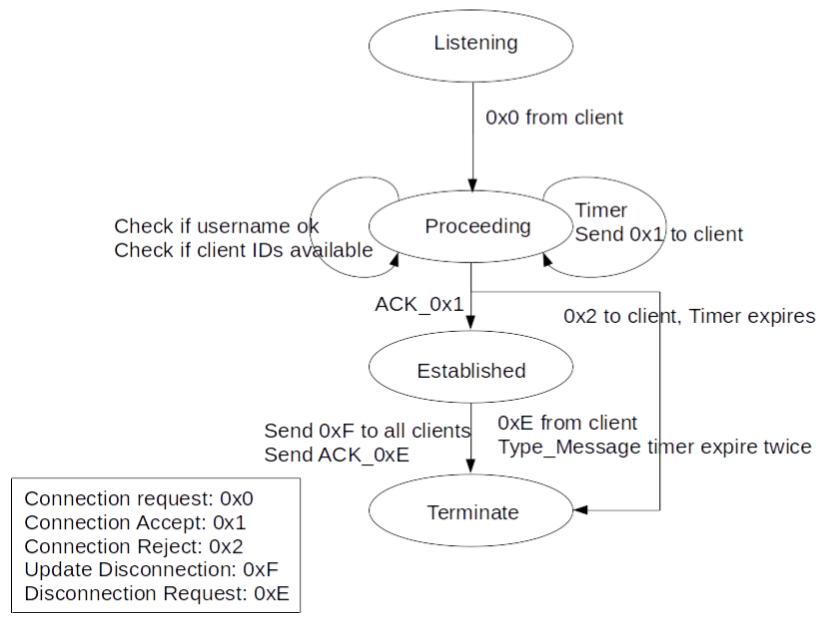
\includegraphics[width=10cm, height=11cm]{Connection-disconnectionFSM.jpg}
\caption{Server Connection-Disconnection Process.}
\label{fig:{Connection-disconnectionFSM}}
\end{figure}


\subsection{Server Messaging Process}
\begin{figure}[H]
\centering
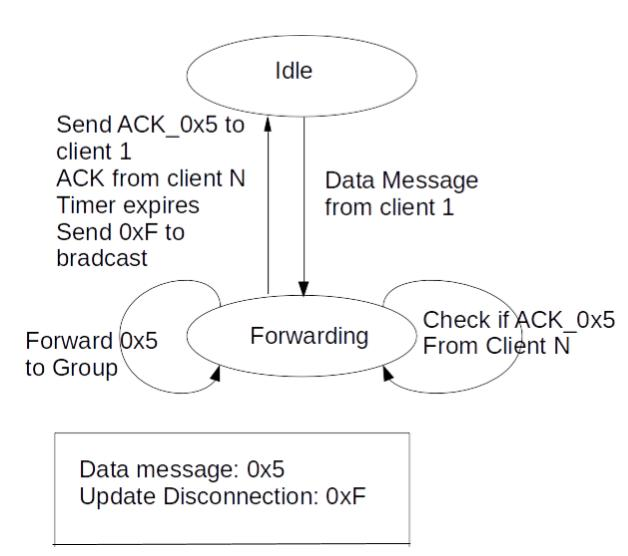
\includegraphics[width=9cm, height=9cm]{MessagingFSM.jpg}
\caption{Server Messaging Process}
\label{fig:{MessagingFSM}}
\end{figure}

\subsection{Server Group Creation Process}
\begin{figure}[H]
\centering
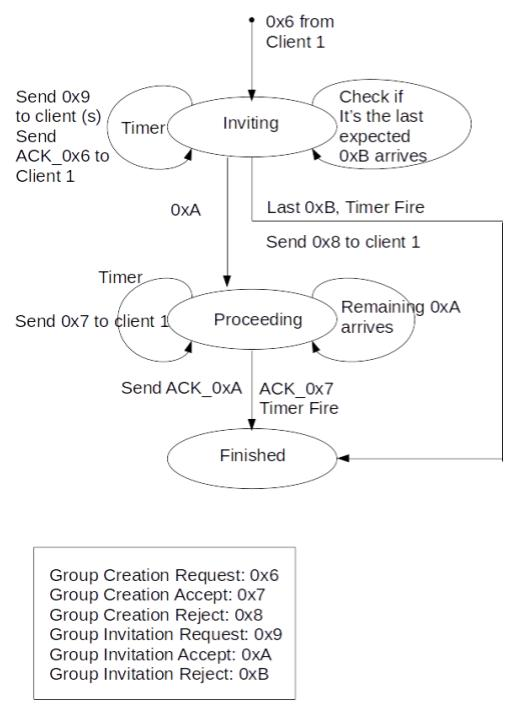
\includegraphics[width=9cm, height=12cm]{GroupCreationFSM.jpg}
\caption{Server Group Creation Process in centralized mode.}
\label{fig:GroupCreationFSM}
\end{figure}



\section{Appendix}


\subsection{Messaging with packet lost special scenario}

During any exchange of messages, packet lost can be present, the protocol handles this situation with a retransmission mechanism. In this example we explain the communication in a centralized mode. When a message is sent by client 1, the server confirms the reception, forwards the message to client 2 and sets a timer that last 500ms, if the packet is lost due to a transmission problem or because of client 2 is not longer available, the sender waits for that time and resends the messages setting up the timer again. Server retries this process and when the last timer, it declares client 2 as disconnected and sends an Update Disconnection message to all client indicating to take off this entry from the list, finally client 2 is removed from the system. This protocols recommends to try 5 attempts before removing the client from the system but it can vary depending on the implementation and the conditions of the network where this protocol will be used.\\

\begin{figure}[H]
\centering
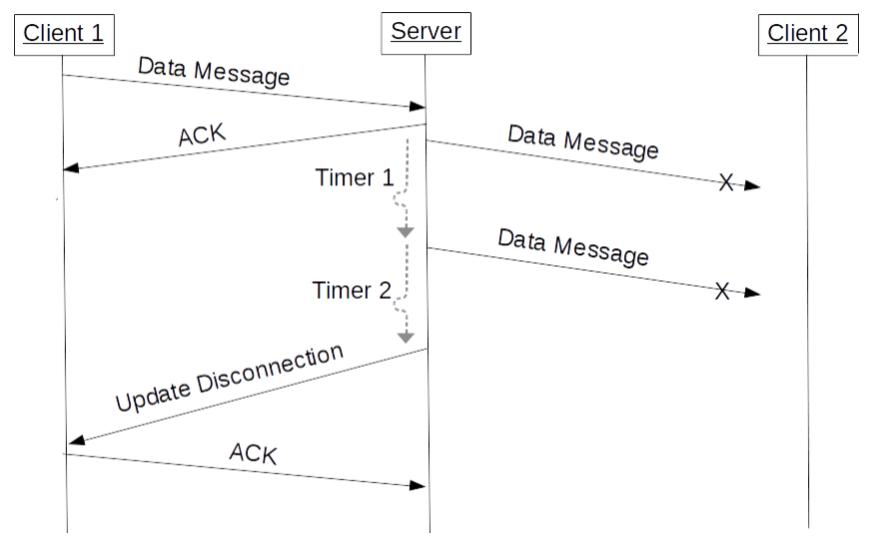
\includegraphics[width=13cm, height=11cm]{Packetlost.jpg}
\caption{Messaging with packet lost scenario in centralized mode.}
\label{fig:Packetlost}
\end{figure}

\bibliographystyle{plain}
\bibliography{references}

\end{document}
